\let\negmedspace\undefined
\let\negthickspace\undefined
\documentclass[journal]{IEEEtran}
\usepackage[a5paper, margin=10mm, onecolumn]{geometry}
%\usepackage{lmodern} % Ensure lmodern is loaded for pdflatex
\usepackage{tfrupee} % Include tfrupee package

\setlength{\headheight}{1cm} % Set the height of the header box
\setlength{\headsep}{0mm}     % Set the distance between the header box and the top of the text

\usepackage{gvv-book}
\usepackage{gvv}
\usepackage{cite}
\usepackage{amsmath,amssymb,amsfonts,amsthm}
\usepackage{algorithmic}
\usepackage{graphicx}
\usepackage{textcomp}
\usepackage{xcolor}
\usepackage{txfonts}
\usepackage{listings}
\usepackage{enumitem}
\usepackage{mathtools}
\usepackage{gensymb}
\usepackage{comment}
\usepackage[breaklinks=true]{hyperref}
\usepackage{tkz-euclide} 
\usepackage{listings}
% \usepackage{gvv}                                        
\def\inputGnumericTable{}                                 
\usepackage[latin1]{inputenc}                                
\usepackage{color}                                            
\usepackage{array}                                            
\usepackage{longtable}                                       
\usepackage{calc}                                             
\usepackage{multirow}                                         
\usepackage{hhline}                                           
\usepackage{ifthen}                                           
\usepackage{lscape}
\begin{document}

\bibliographystyle{IEEEtran}
\vspace{3cm}
\title{9.3.12}
\author{EE24BTECH11028 - Jadhav Rajesh}
% \maketitle
% \newpage
% \bigskip
{\let\newpage\relax\maketitle}

\renewcommand{\thefigure}{\theenumi}
\renewcommand{\thetable}{\theenumi}
\setlength{\intextsep}{10pt} % Space between text and floats


\numberwithin{equation}{enumi}
\numberwithin{figure}{enumi}
\renewcommand{\thetable}{\theenumi}
 \textbf{Question:} Which of the following differential equations has $y = x$ as one of its particular solution?\\
 \begin{align}
 \brak{C}  \frac{d^{2}y}{dx^{2}}-x^{2}\frac{dy}{dx}+xy=0
 \end{align}
                         
 \solution 
  By first principle of derivatives,
  \begin{align}
      y'\brak{t}= \lim_{h \to 0} \frac{y\brak{t+h}-y\brak{t}}{h}
  \end{align}
  \begin{align}
      y\brak{t+h} = y\brak{t}+hy'\brak{t}
  \end{align}
  \begin{align}
  \frac{d^{2}y}{dx^{2}}-x^{2}\frac{dy}{dx}+xy=0
  \end{align}
  Rewriting the given equation , we get:
  \begin{align}
      \frac{d^{2}y}{dx^{2}}=x^{2}\frac{dy}{dx}-xy
  \end{align}
  To solve this equation numeriacally,we apply Euler's method. we start by introducing the following substitution:\\
  Let:
  \begin{align}
      y_{1}=y, y_{2} = \frac{dy}{dx} 
  \end{align}
  Thus, the system become:
  \begin{align}
      y'_{1}=y_{2}
  \end{align}
  \begin{align}
      y'_{2}=x^{2}y_{2}-xy_{1}
  \end{align}
  The system of equation in matrix form:
  \begin{align}
      y'=\myvec{y_{2}\\
                  x^{2}y_{2}-xy_{1}}
  \end{align}
  Using Euler's method, the update formulas become:
  \begin{align}
      y_{1}\brak{x+h}=y_{1}+h\cdot y_{2}
  \end{align}
  \begin{align}
      y_{2}\brak{x+h}=y_{2}\brak{x}+h\cdot\brak{x^{2}y_{2}-xy_{1}}
  \end{align}
  This can expressed in matrix form as:
  \begin{align}
      y_{n+1}=y_{n}+h\myvec{0 && 1\\
                            x && -x^{2}}\cdot y_{n}
  \end{align}
  We will use the initial condition:
  \begin{align}
      y_{1}=1,   y_{2}=0
  \end{align}
  We ,applying Euler's method and iterating.The following plot represent the solution based on these initial condition.
  \begin{figure}[h!]
   \centering
   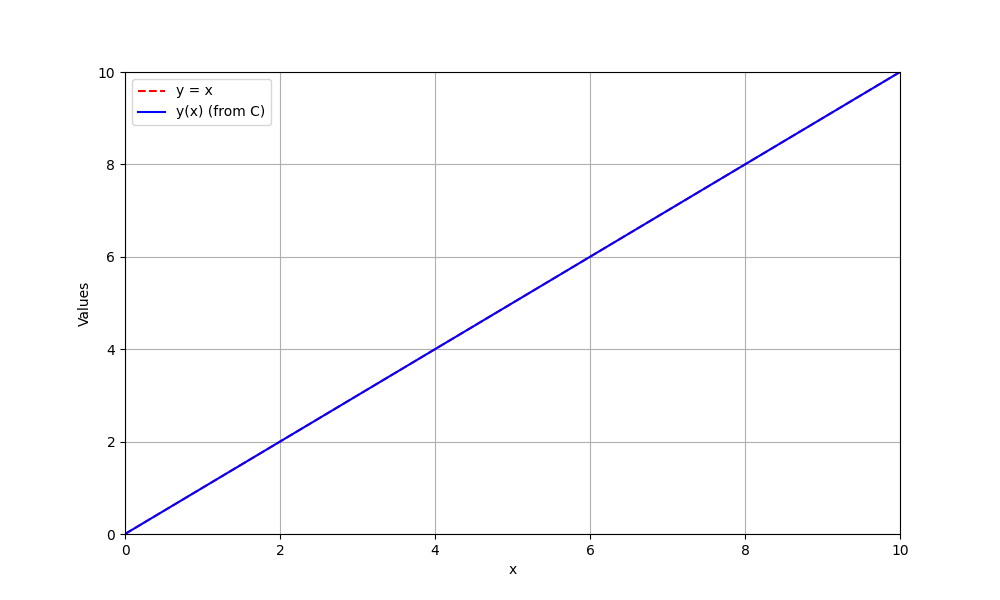
\includegraphics[width=1\columnwidth]{figure/fig.png} 
   \caption{Numerical Solution}
   \label{stemplot}
\end{figure}



\end{document}
